

\documentclass{beamer}
 
\usepackage[utf8]{inputenc}
 
 
%Information to be included in the title page:
\title{Multi-Agent Ethical Planning}
\author{Axel Ind}
\institute{Uni-Freiburg}
\date{\today}
 
 
 
\begin{document}
 
\frame{\titlepage}
%----------------------INTRODUCTION------------------------------------------------
%----------------------------------------------------------------------------------

%----------------------EXAMPLE-----------------------------------------------------
\begin{frame}
\frametitle{Example}
\begin{itemize}
\item Two students (A and B) have a test to study for.
\item They each need a certain textbook from the library. 
\item The library has 2 copies of the textbook, one in English and one in German.
\item Student A speaks both English and German, Student B speaks only English.
\item A arrives at the library early and gets to choose which book he wants first.
\end{itemize}

\end{frame}

 
\begin{frame}
\frametitle{Example: Agent A}
Agent A:
\[
\Pi_A = (V_A, O_A, I_A, \gamma_A, u_A)
\]
\[
O_A = \{ O_{A_{takeEnglish}}, O_{A_{takeGerman}}, O_{A_{doNothing}}\}
\]
\[
O_{A_{takeEnglish}}=(libraryHasEnglish, \lnot libraryHasEnglish \land AhasEnglish)
\]
\[
O_{A_{takeGerman}}=(libraryHasGerman, \lnot libraryHasGerman \land AhasGerman)
\]
\[
O_{A_{doNothing}}=(\top, \top)
\]
\[
I_A = (libraryHasEnglish, libraryHasGerman)
\]
\[
\gamma = (AhasEnglish \lor AhasGerman)
\]

$u_A$: considers ethical evaluation of B's actions.

\end{frame}

\begin{frame}
\frametitle{Example: Agent B}
Agent B:
\[
\Pi_B = (V_B, O_B, I_B, \gamma_B, u_B)
\]
\[
O_B = \{ O_{B_{takeEnglish}}, O_{B_{takeGerman}}, O_{B_{doNothing}}\}
\]
\[
O_{B_{takeEnglish}}=(libraryHasEnglish, \lnot libraryHasEnglish \land BhasEnglish)
\]
\[
O_{B_{takeGerman}}=(libraryHasGerman, \lnot libraryHasGerman \land BhasGerman)
\]
\[
O_{B_{doNothing}}=(\top, \top)
\]
\[
I_B = (libraryHasEnglish, libraryHasGerman)
\]
\[
\gamma = (BhasEnglish)
\]

$u_A$: \textit{does not} consider ethical evaluation of A's actions.
\end{frame}

\begin{frame}
\frametitle{Example: Combined Task}
Combined Task:
\[
\Pi = (V, O, I, \gamma, u, T)
\]
\[
O = (O_A, O_B)
\]
\[
V = V_A \oplus V_B
\]
\[
I = I_A \oplus I_B
\]
\[
\gamma = (\gamma_A, \gamma_B)
\]
\[
u=(u_A, u_B)
\]
$T$: an ordering function to linearise agent actions consistently  (turn taking in this case).
 \end{frame}
 
 
 
\begin{frame}
\frametitle{Flowchart}
\centering 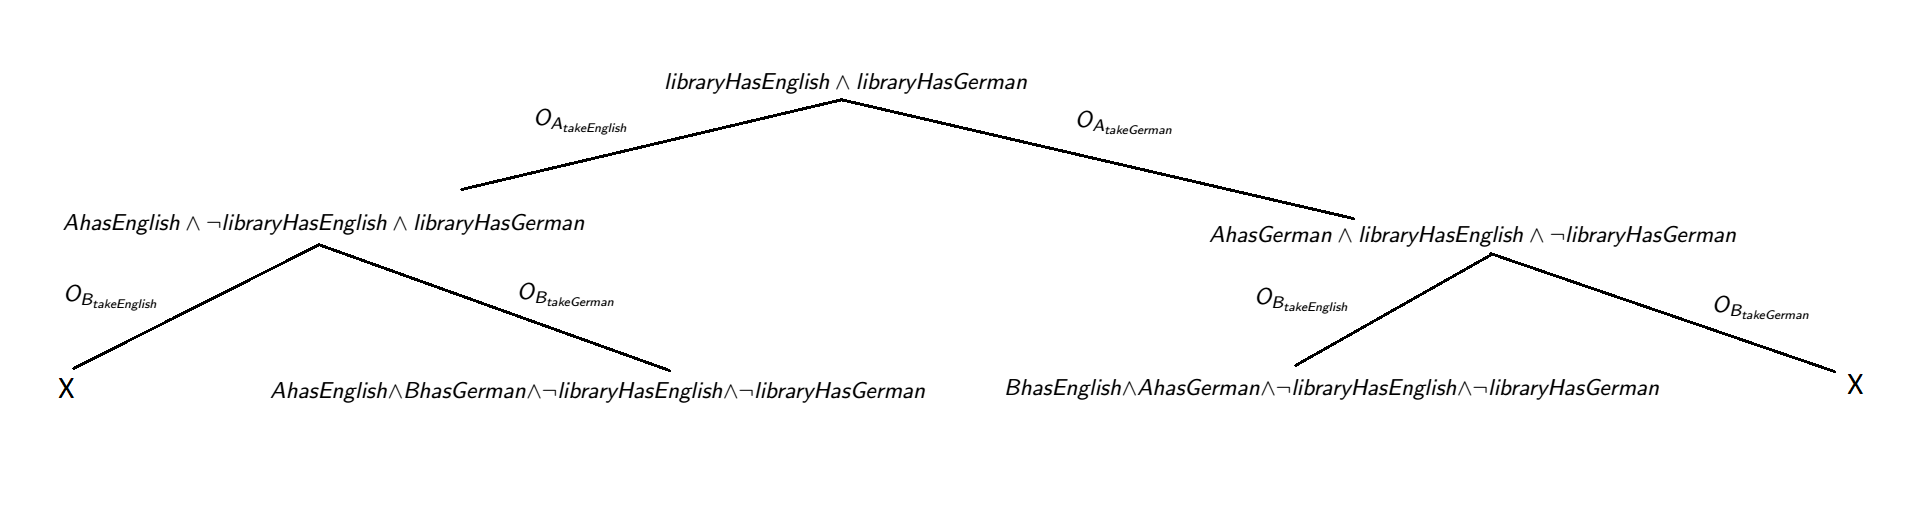
\includegraphics[scale=0.23]{exampleFlowchart}
 \end{frame} 

\begin{frame}
\frametitle{Flowchart}
\centering 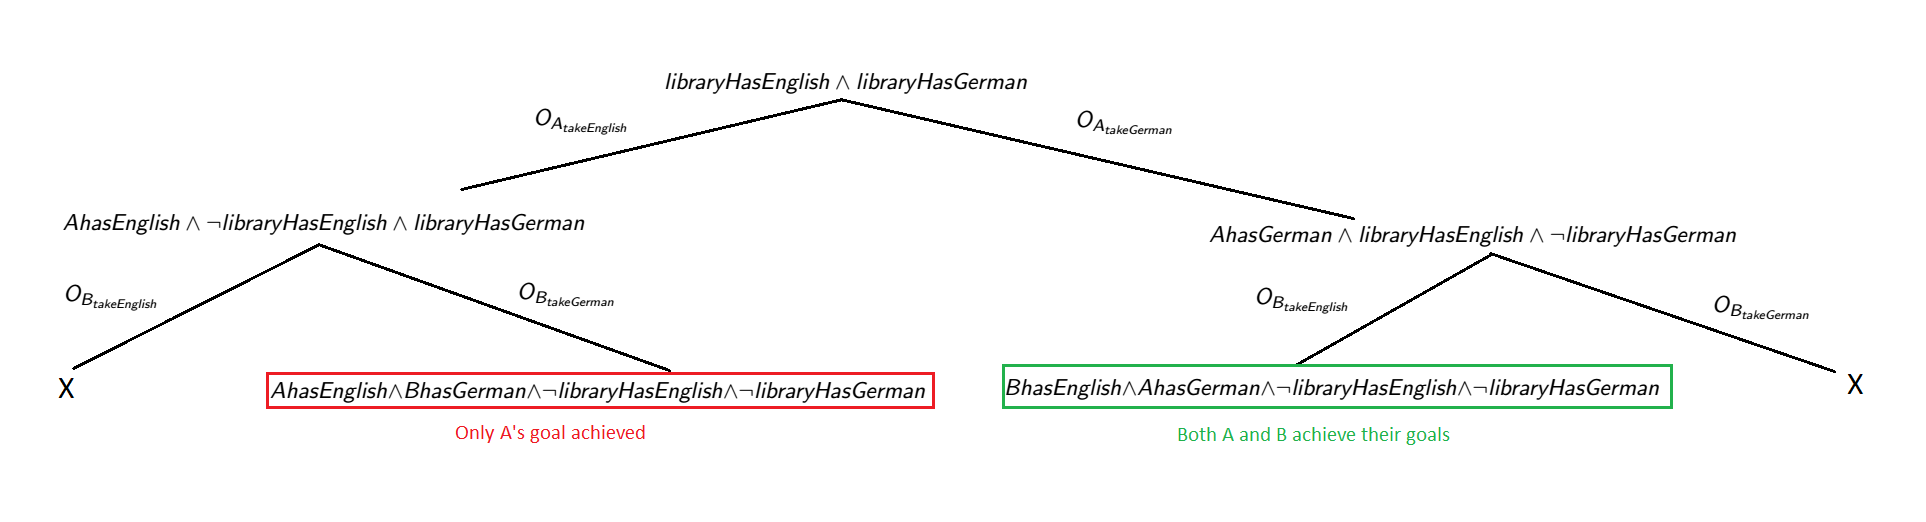
\includegraphics[scale=0.23]{exampleFlowchartAnnotated}

\begin{itemize}
\item Without ethical restrictions of permissable actions, agent A can reach its goal but render agent B's goal unreachable.
\item This is not necessarily bad (e.g. in competitive games), but there are cases where it harms the system as a whole.
\end{itemize}
 \end{frame} 
 
%----------------------Deontological Approach------------------------------------------------- 
\begin{frame}
\frametitle{Deontological Approach}
\begin{itemize}
\item \textit{Actions} labelled \textit{a priori}.
\item Only allow good or morally neutral actions.
\item Morally permissible if: $u(s,a) \geq 0$.
\item For single agent sufficient to simply check if a candidate action has non-negative.
\item For multi-agent case, two possibilities:
\begin{enumerate}
\item Single-agent ethical utility: Consider only the ethical utility of the state-action pair for the acting agent.
\item Agent set ethical utility: Consider ethical utility of the state-action pair of the current agent and \textit{all agents that act after it} until the current agent is able to act again.
\end{enumerate}
\end{itemize}
 \end{frame} 
 
 
 \begin{frame}
\frametitle{Agent Set Ethical Utility}
\begin{itemize}
\item Requires ethical utility labels for other agent actions.
\item If the other agents are random or have unknown $u$, consider worst-case or average-case of their applicable actions.
\item If the other agents $u$ function is known, more complex:
\begin{itemize}
\item If all subsequent agent actions for this turn are morally good or neutral, then the original action is applicable. If all are morally bad or neutral, the action is morally inapplicable. 
\item If both agents follow deontological ethics, and have the same (agent-independent) utility function: it is sufficient to consider the best-case scenario of other agent action selection.
\item In other cases the other agent's actions must be evaluated using their own ethical function to determine what action they will take. Potentially extremely high computational complexity, mitigated by bounded-lookahead.
\item Else possibly heuristic state evaluation based on applicable actions.
\end{itemize} 
\end{itemize}
 \end{frame} 
 
 
\begin{frame}
\frametitle{Deontological Approach Example}
\begin{itemize}
\item We assume that it is ethical for an agent to get a textbook they can read (and therefore pass).
\item We assume that it is unethical to get a textbook you cannot read.
\end{itemize}

Using the definition which relies only on the ethical value of the acting agent's action:
\begin{itemize}
\item A can take either the English or the German book and as both are ethical actions for that agent.
\item B can only take the English book, taking the German is morally impermissible.
\item Thus if A takes the English book ($u_A(I,O_{A_{takeEnglish}})$) it causes B to take an action that is not ethically permissible.
\end{itemize}
\end{frame} 
 
 \begin{frame}
\frametitle{Deontological Approach Example}
Using the definition which relies on the ethical value of the acting agent's action AND all subsequent agent actions until the acting agent is able to act again:
\begin{itemize}
\item A cannot take the English book because it means that the best case for B would still be an unethical action.
\item Thus A must take the German book, and B must then take the English book (both morally permissible).
\item If we allow B to have $O_{B_{doNothing}}$ with no ethical value, the best case for $O_{A_{takeEnglish}}$ becomes a morally permissible action, but the worst and average-case scenarios continue to have expected ethical utility $<0$.
\end{itemize}
@TODO illustrate with images on diagram.
\end{frame} 

%----------------------Utalitarian Approach---------------------------------------------------

 \begin{frame}
\frametitle{Utilitarianism}
\begin{itemize}
\item Consequences matter (state evaluation rather than action evaluation).
\item Goal is that the action which results in the state with the \textbf{highest ethical utility} is taken.
\item Direct relation to game theory.
\item Only difference is that $u_A$ and $u_B$ can evaluate the same state differently.
\item Consider that other agents may not be utilitarian at all.
\end{itemize}
 \end{frame} 


 \begin{frame}
\frametitle{Utilitarianism Cases}
Agent Considerations
\begin{enumerate}
\item Only the acting agent's resulting state matters.
\item Only the state in which A is able to act again matters.
\item All intermediate states until A is able to act again matter.
\end{enumerate}

Search Restrictions
\begin{enumerate}
\item One-step lookahead.
\item Bounded lookahead.
\item Unbounded lookahead.
\end{enumerate}
 \end{frame} 
 
 
 \begin{frame}
\frametitle{Utilitarianism Cases}

\begin{itemize}
\item With:
\begin{enumerate}
\item Only acting agent's state matters.
\item One-step lookahead.
\end{enumerate}
\item It is sufficient to use the average or worst-case utility function of $u_i(s')$ where $s'=app(s,a)$.
\item Constant time.
\end{itemize}

 \end{frame} 
 
 \begin{frame}
\frametitle{Utilitarianism Cases}

\begin{itemize}
\item With:
\begin{enumerate}
\item Only acting agent's state matters.
\item Bounded lookahead.
\end{enumerate}
\item In words: we want to maximize the \textbf{total} return of the acting agent over the $n$ time-steps.
\item Requires knowledge of other agent actions: can use worst, average cases if $u$ of other agents is unknown.
\item If $u$ function of other agents known: if that $u$ values have no dependance on anything but their own state/action/successor state values (i.e. independent of other agents) it's permissible action subset can be computed in constant time. 
\item From this permissible action/state subset can use worst case or average case evaluations in terms of ethical value of resultant states.

\end{itemize}

 \end{frame} 
  
 \begin{frame}
\frametitle{Utilitarianism Cases}
\begin{itemize}
\item With:
\begin{enumerate}
\item Only acting agent's state matters.
\item Bounded lookahead.
\end{enumerate}
\item Generative model.
\end{itemize}

\[
max_{a_i \in A_i} \left( \sum^n_{i=i+numAgents} u(s_i,a_i) \right)
\]

$n$: total number of (action, state) pairs in the bound.
\[
s_i=app(s_{i-1},a_{i-1})
\]
 \end{frame} 
 
 
 \begin{frame}
\frametitle{Utilitarianism Cases}
\begin{itemize}
\item With:
\begin{enumerate}
\item Only the state in which A is able to act again matters.
\item One-step lookahead.
\end{enumerate}
\item For agent $k$:
\end{itemize}
\[
O_k = max_{{a_i \in O_{k+1}}} max_{a_i \in O_k}   
\]
\[
O_{k+n} = u(s')
\]

\begin{itemize}
\item Very high computational complexity.
\item Can make use of properties of the $u$ function of other agents to only search permissible states for those agents.
\end{itemize}

 \end{frame} 
 
%----------------------Do No Harm--------------------------------------------------- 
 \begin{frame}
\frametitle{Do No Harm}
\begin{itemize}
\item Removing any subset of the actions in the sequence of actions would not prevent any bad variable assignments.
\item Uses $u(v=d)$ to give an ethical utility to individual variables.
\end{itemize}

For the library example:
\begin{itemize}
\item The bad effect of B failing only happens when A takes the English book.
\item The bad effect of A failing only happens if B takes both books.
\end{itemize}
 \end{frame} 
 
 
 \begin{frame}
\frametitle{Do No Harm Cases}

Lookahead
\begin{itemize}
\item One-step lookahead.
\item Bounded lookahead.
\item Unbounded lookahead.
\end{itemize}

Agent evaluations
\begin{itemize}
\item Evaluate only the final state $s'$ before the acting agent is able to act again.
\item Evaluate only the $s'$ states resulting from the acting agent's actions.
\item Evaluate the $s'$ states resulting from every agent's actions.
\end{itemize}

 \end{frame} 
 

%----------------------EXTENSIONS------------------------------------------------
%----------------------------------------------------------------------------------

%----------------------Extending Pi----------------------------------------------------- 
 \begin{frame}
\frametitle{Extensions}
Previously:
\[
\Pi = (V, O, I, \gamma, u, T)
\]

Now Define:
\[
\Pi = (V, O, I, \gamma, u, T, V, W)
\]

\begin{itemize}
\item $W$ assigns an agent, or set of agents to some set (or subset of sets) $w$.
\item $u$ is now an order list of \textit{utility vectors}.
\item $V$ is an ordering function that gives precedent to classes in $W$.
\end{itemize}

 \end{frame} 
 
\begin{frame}
\frametitle{Extensions Motivation}
\begin{itemize}
\item Our ethical dealings with people are not uniform.
\item We may apply utilitarian ethics wrt. our own happiness, do-no-harm ethics to friends, Deontic ethics to strangers, and inversions of any of these to our enemies.
\item We may even combine these ethics and decide to act with utilitarian ethics provided none of the actions we take are illegal (deontically impermissible).
\item So instead of assigning ethical utility according to only a single principle, it is possible to determine the effect of a single action or consequence in terms of multiple ethical principals at once.
\end{itemize}
 \end{frame}  
 
 
 
\begin{frame}
\frametitle{Extensions}
\begin{itemize}

\item Thus, $u$ becomes a set of vectors of utility functions corresponding to how each agent interprets each event wrt. to its ethical interpretations.
\item $W$ maps (agent, action, state, variables) tuples or tuple subsets to their classes (e.g. friend, enemy, self). This determines which functions within $u$ will ethically evaluate the tuple.
\item $V$ provides an ordering for the precedence (importance) of different ethical systems. Thus it may specify that utilitarian ethics are superseded by deontic ethics and so only states that meet the deontic criteria are candidate states for the utilitarian evaluation.
\item $V$ is not essential to the planning task, but provides a consistent way to evaluate tuples. Without it final states would not be consistent across runs.
\end{itemize}
 \end{frame}
 
 
 \begin{frame}
\frametitle{Extensions: Trolley Problem}
\begin{itemize}
\item Can divide people on track into 6 distinct agents (all with action $O_{doNothing}$).
\item The actor pulling the lever is also an agent.
\item $W$ may place the acting agent into its own distinct group (actor).
\item $W$ also places all track agents into a group (victim).
\item $u$ Ethical value of actions can now be evaluated (as normal) by considering the moral effect of agents according the ethical system under consideration.
\end{itemize}
\end{frame}

 \begin{frame}
\frametitle{Extensions: Trolley Problem with Friend}
\begin{itemize}
\item Consider now that the one person on the track is your friend.
\item You consider the ethical effect of actions affecting your friend to be of greater significance than those affecting normal victims.
\item $W$ still places all track agents into a group (victim).
\item $W$ also places your friend into a special group (friend).
\item $V$ allocates the friend class a greater priority.

\end{itemize}

 \end{frame}
 
 
 \begin{frame}
\frametitle{Extensions: Trolley Problem with Friend}
\begin{itemize}
\item Now ethical evaluation of the states will first generate only candidate states that are not ethically harmful to the friend class. From these candidate states that are not harmful to the victim class can be generated.
\item If no such state/action exists for the victim class, but does for the friend, and an action is forced, then the idea of \textit{the least unethical choice} comes into effect.
\end{itemize}
 \end{frame}
 
 
 \begin{frame}
\frametitle{Extensions}
 \end{frame}
  
  
  \begin{frame}
\frametitle{Extensions}
 \end{frame}
 
 
 \begin{frame}
\frametitle{Extensions}
 \end{frame}
 
 
 \begin{frame}
\frametitle{Extensions}
 \end{frame}
 
 
 \begin{frame}
\frametitle{Extensions}
 \end{frame}
 
 
 
 
 
 
 
 
 
 
 
 
 
 
 
 
\begin{frame}
\frametitle{DELETE ME}

\[
libraryHasEnglish \land libraryHasGerman
\]
\[
AhasEnglish \land \lnot libraryHasEnglish \land libraryHasGerman
\]
\[
BhasEnglish \land \lnot libraryHasEnglish \land libraryHasGerman
\]
\[
AhasGerman \land libraryHasEnglish \land \lnot libraryHasGerman
\]
\[
BhasGerman \land libraryHasEnglish \land \lnot libraryHasGerman
\]
\[
AhasEnglish \land BhasGerman \land \lnot libraryHasEnglish \land \lnot libraryHasGerman
\]
\[
BhasEnglish \land AhasGerman \land \lnot libraryHasEnglish \land \lnot libraryHasGerman
\]
\[
AhasEnglish \land AhasGerman \land \lnot libraryHasEnglish \land \lnot libraryHasGerman
\]
\[
BhasEnglish \land BhasGerman \land \lnot libraryHasEnglish \land \lnot libraryHasGerman
\]

 \end{frame}
\end{document}

